\documentclass{Support}

\begin{document}

\renewcommand{\myTitle}{Théorie des langages- IN406}
\renewcommand{\MyAuthor}{Evaluation d'expressions booléennes}
\renewcommand{\MyDepartment}{Zeyneb Bouabdallaoui, Nicolas Fond}
\renewcommand{\ID}{21904931 / 21908626}
\maketitle

\vspace{-1.9em}\noindent\rule{\textwidth}{1pt}
\onehalfspacing

\section*{Introduction}
Ce projet consiste à évaluer des expressions booléennes en C à l'aide d'automates à piles. Nous expliquerons ici les automates construits ainsi qu'une bref description du code.

\section{Reconnaissance par automate}
Le but de cette partie est de construire un automate à pile permettant de reconnaître une expression booléenne. Chaque élément de l'expression devient ici un \textit{token} et l'expression booléenne entière un mot. Pour construire l'automate, nous pouvons tout d'abord nous intéresser aux propriétés de chaque type de l'expression. Nous allons tout d'abord regarder quels sont les éléments qui peuvent venir avant et après un élément. Par exemple un 1, soit une constante, ne peut avoir une parenthèse ouvrante après lui. On peut alors émettre une liste de conditions qui indiquent quels sont les prédécesseurs et les successeurs possibles d'un élément donné. De ce fait, on crée une vérification locale de chaque élément:

\vspace{0,4cm}
\hspace*{-1.9cm}
\begin{tabular}{|m{3,6cm}||m{2cm}|m{3cm}|m{2,5cm}|m{2,5cm}|m{2cm}|} 
    \hline
      & Constante $0$, $1$  & Opérateur unaire $+, \bullet , \Rightarrow , \iff, +$ & Parenthèse ouvrante $($ & parenthèse fermante $)$  & Opérateur unaire $NON$ \\
    \hline
     Constante           &   &  X  &  X  &    & X \\
    \hline
     Opérateur binaire   & X &     &     &  X &  \\
    \hline
     Parenthèse ouvrante &   & X   & X   &    & X  \\
    \hline
     Parenthèse fermante & X &     &     & X  &  \\
    \hline
     Opérateur unaire    &   & X   & X   &    &  \\
    \hline
\end{tabular}

\vspace{0,4cm}
Chaque croix sur ce tableau signifie que l'élément $a$ est prédécesseur de l'élément $b$ et donc que $b$ est successeur de $a$. Le tableau se lit de la façon suivante : si on veut connaître les prédécesseurs, il suffit de regarder sur la colonne en abscisse l'élément voulu puis à chaque croix rencontrée dans la colonne correspond un prédécesseur. De la même manière, si on veut connaître les successeurs d'un élément, on regarde en ordonnée où se situe l'élément souhaité puis à chaque croix rencontrée dans la ligne correspond un successeur. Ce tableau nous sera très utile pour construire l'automate.

Maintenant que nous connaissons les contraintes pour chaque élément, nous pouvons construire les automates qui nous permettront de construire l'automate final comprenant les expressions booléennes.

Tous les automates seront des automates à reconnaissance par pile vide. On notera $\delta$ la pile vide. Pour clarifier les automates, chaque transition sera marquée sans parenthèses, un saut de ligne indiquera qu'on se trouve sur une autre transition.

On notera $a$ l'ensemble qui comprend les constantes $1$ et $0$ et $b$ l'ensemble qui comprend les opérateurs binaires $\Rightarrow$, $\bullet$, $\iff$ et $+$. L'opérateur unaire sera noté $n$ et les parenthèses $($ et $)$. On a donc : 
$$
a= \{1,0 \} \ ; \ b = \{\Rightarrow, \iff, +, \bullet \} 
$$
Chaque transition sera représentée sous cette forme : 
$$
x, Y \rightarrow X
$$
Cela signifie que si la tête de lecture du mot lit un $x$ et que la pile contient un $Y$, alors $Y$ devient $X$. Les automates suivants sont non déterministes.
\subsection{Automate 1}
Commençons simplement par un automate qui reconnaît les expressions booléennes contenant uniquement des constantes et des opérateurs binaires. Soit en version simplifier une alternance de $a$ et de $b$ où $a$ doit commencer et finir l'expression. Par exemple $ababa$ est valide.  Les mots $a$, $abb$, $abab$ ou $aaba$ ne ne sont pas valides et ne seront donc pas reconnu par l'automate. L'idée est de créer une pile permettant de stocker le prédécesseur de l'élément actuel. Ainsi, en connaissant le prédécesseur (en se servant du tableau), on peut créer des transitions possibles après ce token. La pile nous servira uniquement à regarder quel était le prédécesseur du token actuel. On crée donc une boucle qui permettra de prendre autant de tokens qu'il y a dans le mot.

\begin{center}
\begin{tikzpicture}[scale=0.2]
\tikzstyle{every node}+=[inner sep=0pt]
\draw [black] (13.5,-29.3) circle (3);
\draw (13.5,-29.3) node {$q_0$};
\draw [black] (36.8,-12.8) circle (3);
\draw (36.8,-12.8) node {$q_1$};
\draw [black] (36.8,-46) circle (3);
\draw (36.8,-46) node {$q_2$};
\draw [black] (14.902,-26.649) arc (149.13708:101.4717:28.707);
\fill [black] (33.83,-13.24) -- (32.95,-12.91) -- (33.15,-13.89);
\draw (18.89,-17.45) node [above, text width=2cm] {$a,B\rightarrow A$ $a, \delta \rightarrow A$};
\draw [black] (15.94,-31.05) -- (34.36,-44.25);
\fill [black] (34.36,-44.25) -- (34,-43.38) -- (33.42,-44.19);
\draw (20.67,-38.15) node [below] {$a,B\rightarrow\varepsilon$};
\draw [black] (6.5,-29.3) -- (10.5,-29.3);
\fill [black] (10.5,-29.3) -- (9.7,-28.8) -- (9.7,-29.8);
\draw [black] (35.496,-15.5) arc (-28.97146:-80.41976:26.843);
\fill [black] (16.48,-28.97) -- (17.35,-29.33) -- (17.19,-28.34);
\draw (31.59,-24.9) node [below] {$b,A\rightarrow B$};
\end{tikzpicture}
\end{center}

\subsubsection*{Construction de l'automate}
Si l'automate lit un $a$, on empilera $A$ pour le mémoriser. Pour passer à l'état suivant, le token d'après est obligatoirement un $b$, on vérifie alors dans cette transition si la valeur précédente est bien $a$ et on remplace le $A$ de la pile par un $B$. Une fois $B$ dans la pile, la transition suivante est obligatoirement un $a$. On a alors deux choix : 
\begin{itemize}
    \item La constante $a$ est le dernier token du mot : on ira donc dans un état qui videra la pile et le mot sera accepté.
    \item La constante $a$ n'est pas le denier token du mot : on refait un tour de boucle comme vu dans le paragraphe précédent.
\end{itemize}

\subsection{Automate 2}
À partir de l'automate précédent, on peut créer l'automate qui reconnaît les expressions booléennes sans les parenthèses. On a donc l'opérateur unaire qui vient s'ajouter à notre automate. Cet opérateur n'est pas très compliqué à implémenter dans l'automate puisqu'il n'a qu'un prédécesseur et un successeur (sans les parenthèses). Il faudra donc prêter attention aux opérateurs unaires quand on implémentera les parenthèses à l'automate.

L'idée est sensiblement la même que l'automate 1 à la différence que l'opérateur unaire peut se positionner avant un $a$ (soit une constante) et après un $b$ (soit un opérateur binaire). Il y aura donc une nouvelle transition de $q_0$ à $q_1$ pour gérer les sous mots $...+NON...$ et une nouvelle transition de $q_1$ à $q_1$ qui viendra ajouter à la pile le $a$ qui vient obligatoirement après un opérateur unaire. Enfin, une transition de $q_1$ à $q_2$ a été ajoutée pour prendre en compte les sous mots du type $NON0$.

\begin{center}
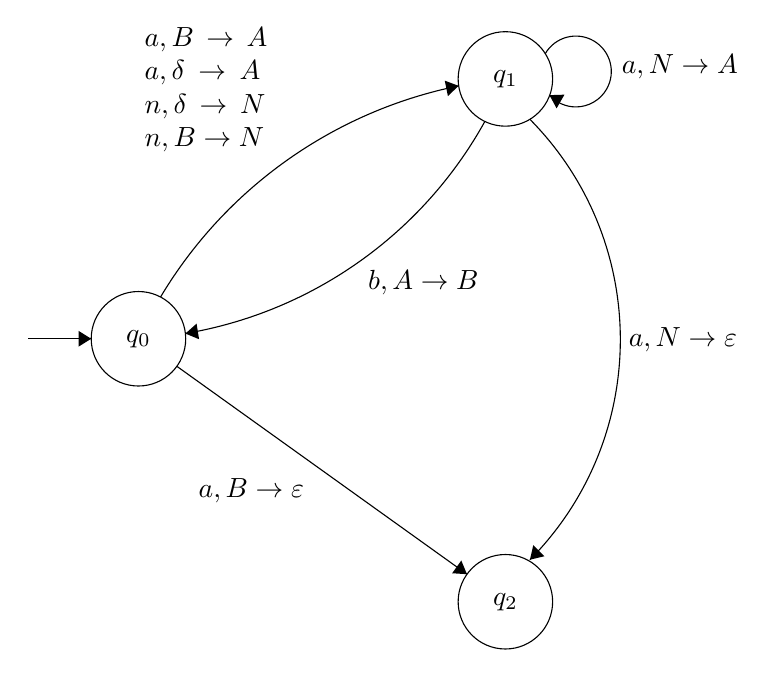
\begin{tikzpicture}[scale=0.2]
\tikzstyle{every node}+=[inner sep=0pt]
\draw [black] (13.5,-29.3) circle (3);
\draw (13.5,-29.3) node {$q_0$};
\draw [black] (36.8,-12.8) circle (3);
\draw (36.8,-12.8) node {$q_1$};
\draw [black] (36.8,-46) circle (3);
\draw (36.8,-46) node {$q_2$};
\draw [black] (14.902,-26.649) arc (149.13708:101.4717:28.707);
\fill [black] (33.83,-13.24) -- (32.95,-12.91) -- (33.15,-13.89);
%transition q0,q1
\draw (18.89,-17.45) node [above, text width=2cm] {$a,B\rightarrow A$ $a, \delta \rightarrow A$ $n,\delta \rightarrow N$ $n, B\rightarrow N$};
\draw [black] (15.94,-31.05) -- (34.36,-44.25);

\fill [black] (34.36,-44.25) -- (34,-43.38) -- (33.42,-44.19);
%transition q0 q2
\draw (20.67,-38.15) node [below] {$a,B\rightarrow\varepsilon$};
\draw [black] (6.5,-29.3) -- (10.5,-29.3);
\fill [black] (10.5,-29.3) -- (9.7,-28.8) -- (9.7,-29.8);
\draw [black] (35.496,-15.5) arc (-28.97146:-80.41976:26.843);
\fill [black] (16.48,-28.97) -- (17.35,-29.33) -- (17.19,-28.34);
% transition q1 q0
\draw (31.59,-24.9) node [below] {$b,A\rightarrow B$};

\draw [black] (39.327,-11.204) arc (150.00901:-137.99099:2.25);
%transition q1 q1
\draw (44.16,-12) node [right] {$a,N\rightarrow A$};
\fill [black] (39.6,-13.83) -- (40.05,-14.67) -- (40.55,-13.8);

\draw [black] (38.36,-15.368) arc (44.6372:-44.6372:19.9);
\fill [black] (38.36,-43.33) -- (39.28,-43.11) -- (38.57,-42.41);
\draw (44.6,-29.35) node [right] {$a,N\rightarrow \varepsilon$};
\end{tikzpicture}
\end{center}

\subsection{Automate final}
Les parenthèses sont ici gérées avec une autre pile qui empilera les parenthèses ouvrantes. À chaque parenthèse fermante rencontrée, on dépilera la parenthèse ouvrante mis au préalable. De ce fait, on vérifie que chaque parenthèse ouvrante se ferme. Si toutes sont fermées, alors la pile sera vide en fin de parcours. Si ce n'est pas le cas, alors la pile ne sera pas vide et le mot ne sera pas reconnu par l'automate.

La gestion des parenthèses nécessite d'ajouter deux boucles. Une à l'état $q_0$ et une à l'état $q_1$. Celle à l'état $q_0$ empile les parenthèses ouvrantes à chaque parenthèse ouvrante rencontrée. Celle à l'état $q_1$ dépile les parenthèses ouvrantes à chaque parenthèse fermante rencontrée.

La transition de $q_1$ à $q_1$ permet aussi de gérer les parenthèses après les constantes.
La pile contenant les opérateurs unaires et binaires ainsi que les constantes est représentée en \textcolor{Orange}{orange} et la pile contenant les parenthèses est représentée en \textcolor{Blue}{bleu}.

\begin{center}
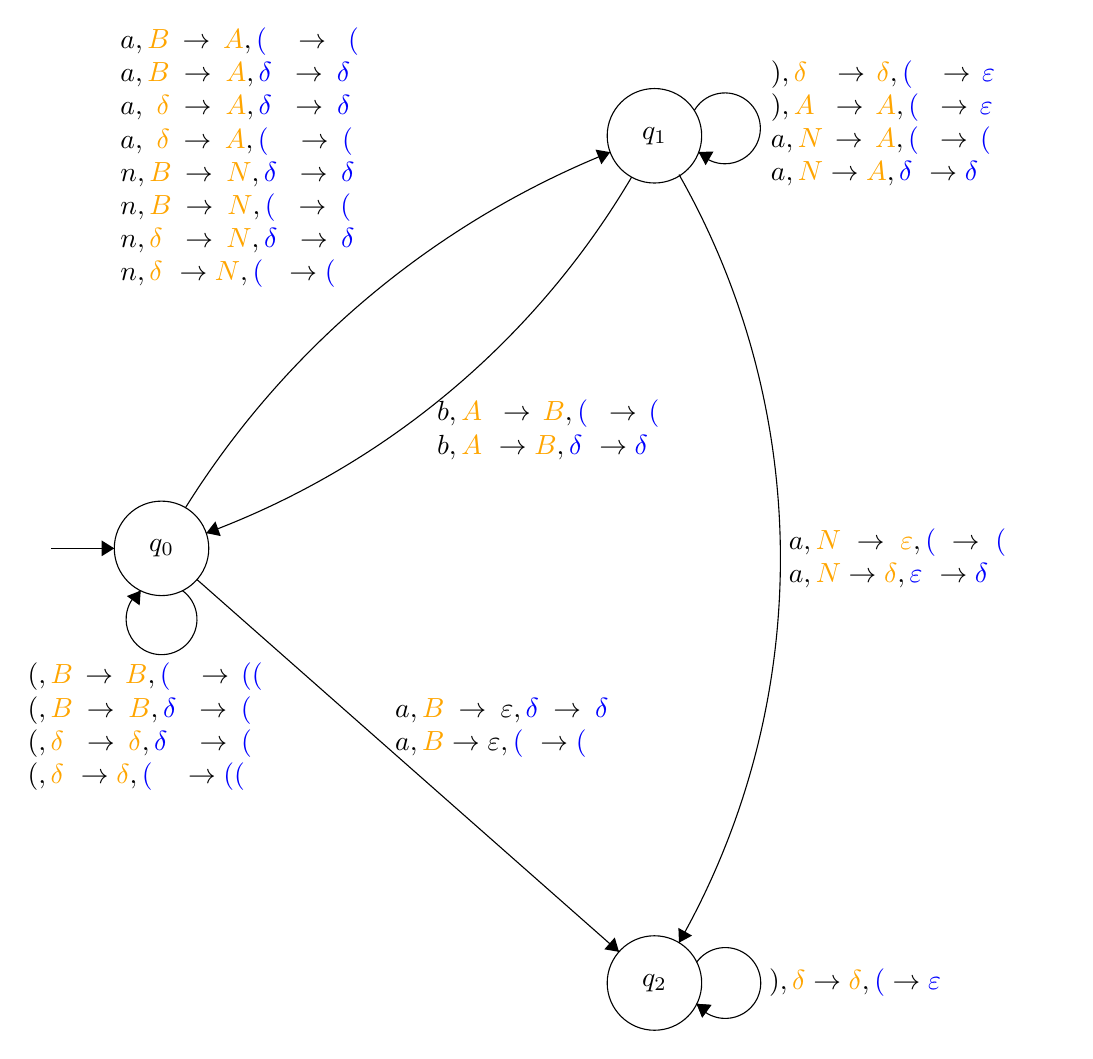
\begin{tikzpicture}[scale=0.2]
\tikzstyle{every node}+=[inner sep=0pt]
\draw [black] (13.5,-29.3) circle (3);
\draw (13.5,-29.3) node {$q_0$};
\draw [black] (44.8,-3.1) circle (3);
\draw (44.8,-3.1) node {$q_1$};
\draw [black] (44.8,-56.9) circle (3);
\draw (44.8,-56.9) node {$q_2$};
\draw [black] (15.022,-26.715) arc (147.99086:111.87189:56.718);
\fill [black] (41.99,-4.14) -- (41.06,-3.98) -- (41.43,-4.91);

%q0 q1
\draw (19.64,-12.79) node [above, text width=3.5cm] {$a,\textcolor{Orange}{B}\rightarrow \textcolor{Orange}{A}, \textcolor{Blue}{(}\ \ \rightarrow\  \textcolor{Blue}{(}$
                                                     $a,\textcolor{Orange}{B}\rightarrow \textcolor{Orange}{A},\textcolor{Blue}{\delta} \ \rightarrow \textcolor{Blue}{\delta}$
                                                     $a,\ \textcolor{Orange}{\delta} \rightarrow \textcolor{Orange}{A}, \textcolor{Blue}{\delta} \ \rightarrow \textcolor{Blue}{\delta}$
                                                     $a, \ \textcolor{Orange}{\delta} \rightarrow \textcolor{Orange}{A}, \textcolor{Blue}{(}\ \ \rightarrow \textcolor{Blue}{(}$
                                                     $n,\textcolor{Orange}{B}\rightarrow \textcolor{Orange}{N}, \textcolor{Blue}{\delta} \ \rightarrow \textcolor{Blue}{\delta}$
                                                     $n,\textcolor{Orange}{B} \rightarrow \textcolor{Orange}{N}, \textcolor{Blue}{(} \ \rightarrow\textcolor{Blue}{(}$
                                                     $n, \textcolor{Orange}{\delta} \ \rightarrow \textcolor{Orange}{N}, \textcolor{Blue}{\delta} \ \rightarrow \textcolor{Blue}{\delta}$
                                                     $n, \textcolor{Orange}{\delta} \ \rightarrow \textcolor{Orange}{N},\textcolor{Blue}{(}\ \ \rightarrow \textcolor{Blue}{(}$};
                                                     
\draw [black] (15.75,-31.28) -- (42.55,-54.92);
\fill [black] (42.55,-54.92) -- (42.28,-54.01) -- (41.62,-54.76);

%q0 q2
\draw (36.59,-42.61) node [above, text width=3.3cm] {$a,\textcolor{Orange}{B}\rightarrow\varepsilon,\textcolor{Blue}{\delta}\rightarrow \textcolor{Blue}{\delta}$
                                                     $a ,\textcolor{Orange}{B}\rightarrow\varepsilon,\textcolor{Blue}{(}\  \rightarrow\textcolor{Blue}{(}$};
                                                     
\draw [black] (6.5,-29.3) -- (10.5,-29.3);
\fill [black] (10.5,-29.3) -- (9.7,-28.8) -- (9.7,-29.8);
\draw [black] (43.35,-5.726) arc (-30.53994:-69.59731:52.686);
\fill [black] (16.34,-28.33) -- (17.26,-28.52) -- (16.92,-27.59);

%q1 q0
\draw (39,-19.85) node [below, text width=3.2cm] {$b,\textcolor{Orange}{A}\ \rightarrow \textcolor{Orange}{B},\textcolor{Blue}{(} \  \rightarrow \textcolor{Blue}{(}$
                                                     $b,\textcolor{Orange}{A}\ \rightarrow \textcolor{Orange}{B}, \textcolor{Blue}{\delta} \ \rightarrow \textcolor{Blue}{\delta}$};
                                                     
\draw [black] (47.327,-1.504) arc (150.00901:-137.99099:2.25);

%q1 q1
\draw (52.16,-2.3) node [right, text width=3.2cm] {
                                 $), \textcolor{Orange}{\delta} \ \ \rightarrow \textcolor{Orange}{\delta}, \textcolor{Blue}{(}\ \ \rightarrow \textcolor{Blue}{\varepsilon}$
                                 $), \textcolor{Orange}{A} \ \rightarrow \textcolor{Orange}{A}, \textcolor{Blue}{(} \ \rightarrow \textcolor{Blue}{\varepsilon}$
                                 $a, \textcolor{Orange}{N} \rightarrow \textcolor{Orange}{A}, \textcolor{Blue}{(}\ \rightarrow \textcolor{Blue}{(}$
                                 $a, \textcolor{Orange}{N} \rightarrow \textcolor{Orange}{A}, \textcolor{Blue}{\delta} \ \rightarrow \textcolor{Blue}{ \delta}$};
                                 
\fill [black] (47.6,-4.13) -- (48.05,-4.97) -- (48.55,-4.1);
\draw [black] (14.823,-31.98) arc (54:-234:2.25);

%q0 q0
\draw (13.5,-36.55) node [below, text width=3.4cm] {
$(, \textcolor{Orange}{B}\rightarrow \textcolor{Orange}{B}, \textcolor{Blue}{(} \ \ \rightarrow \textcolor{Blue}{((}$
$(, \textcolor{Orange}{B}\rightarrow \textcolor{Orange}{B}, \textcolor{Blue}{\delta} \ \rightarrow\textcolor{Blue}{(}$
$(, \textcolor{Orange}{\delta} \ \rightarrow \textcolor{Orange}{\delta},\textcolor{Blue}{\delta} \ \ \rightarrow\textcolor{Blue}{(}$
$(, \textcolor{Orange}{\delta} \ \rightarrow \textcolor{Orange}{\delta},\textcolor{Blue}{(} \ \ \ \rightarrow \textcolor{Blue}{(( }$};

\fill [black] (12.18,-31.98) -- (11.3,-32.33) -- (12.11,-32.92);
\draw [black] (47.48,-55.577) arc (144:-144:2.25);

%q2 q2
\draw (52.05,-56.9) node [right, text width=3.5cm] {                        $),\textcolor{Orange}{\delta}\rightarrow \textcolor{Orange}{\delta}, \textcolor{Blue}{(} \rightarrow\textcolor{Blue}{\varepsilon}$};
\fill [black] (47.48,-58.22) -- (47.83,-59.1) -- (48.42,-58.29);

\fill [black] (47.48,-58.22) -- (47.83,-59.1) -- (48.42,-58.29);
\draw [black] (46.36,-5.562) arc (29.58748:-29.58748:49.393);
\fill [black] (46.36,-54.34) -- (47.19,-53.89) -- (46.32,-53.4);
\draw (53.3,-29.95) node [right, text width=3.5cm] {$a,\textcolor{Orange}{N}\rightarrow\textcolor{Orange}{\varepsilon},\textcolor{Blue}{(}\rightarrow\textcolor{Blue}{(}$
$a, \textcolor{Orange}{N} \rightarrow \textcolor{Orange}{\delta}, \textcolor{Blue}{\varepsilon} \ \rightarrow\textcolor{Blue}{\delta}$};

\end{tikzpicture}
\end{center}

\subsubsection*{Description formelle de l'automate}
\noindent
$\mathcal A = (\Epsilon, Q,q_0, \Gamma,\delta,F,T$) \\
\noindent
$\Sigma = \{a,b,n,(,)\} \\$
$Q = \{q_0,q_1,q_2\} \\$
$\Gamma = \{A,B,N,(,)\} \\$
$F = \mbox{Reconnaissance par pile vide} \\$
$
    T=
      \begin{Bmatrix} 
        q_0,\ (,\  B,\ (,\ q_0, \ B,\ (( \\
        q_0,\  (,\ \ \delta,\  \delta,\  \ q_0,\ \delta,\ ( \\
        q_0,\ (,\ B,\ (,\ q_0,\ \delta,\ (( \\
        q_0,\ a,\ B,\ (,\ q_1,\ A,\ ( \\
        q_0,\ a,\ B,\ \delta,\ q_1,\ A,\ \delta \\
        q_0,\ a,\ \delta,\ \delta,\ q_1,\ A,\ \delta \\
        q_0,\ a,\ \delta,\ (,\ q_1,\ A,\ ( \\
        q_0,\ n,\ B,\ \delta,\ q_1,\ N,\ \delta\\
        q_0,\ n,\ B,\ (,\ q_1,\ N,\ (\\
        q_0,\ n,\ \delta,\ \delta,\ q_1,\ N,\ \delta\\
        q_0,\ n,\ \delta,\ (,\ q_1,\ N,\ (\\
        q_0,\ a,\ B,\ \delta,\ q_2,\ \varepsilon,\ \delta \\
        q_0,\ a,\ B,\ (,\ q_2,\ \varepsilon,\ ( \\
        q_1,\ ),\ \delta,\ (,\ q_1,\ \delta,\ \epsilon \\
        q_1,\ ),\ A,\ (,\ q_1,\ A,\ \epsilon \\
        q_1,\ a,\ N,\ (,\ q_1,\ A,\ ( \\
        q_1,\ a,\ N,\ \delta,\ q_1,\ A,\ \delta \\
        q_1,\ b,\ A,\ (,\ q_0,\ B,\ ( \\
        q_1,\ b,\ A,\ \delta,\ q_0,\ B,\ \delta \\
        q_1,\ a,\ N,\ (,\ q_2,\ \varepsilon,( \\
        q_1,\ a,\ N,\ \varepsilon,\ q_2,\ \delta,\ \delta \\
        q_2,\ ),\ \delta,\ (,\ q_2,\ \delta,\ \varepsilon \\
       \end{Bmatrix}
$


\section{Fonction principale du programme}
Pour rappel, l'idée générale du projet est de mettre en argument une expression booléenne à notre programme et qu'il en ressort le résultat. Pour cela, on créé une liste de \textit{tokens} qui prend tous les éléments de l'expression booléenne. On réalise ensuite notre arbre en fonction de la liste de \textit{token}. Finalement on calcule le résultat de notre expression à partir de l'arbre qui lui correspond. Le résultat est ensuite affiché sur le terminal.

\section{Affichage}
Le programme possède un affichage simple montrant qu'il a bien pris en compte chaque \textit{token} et un affichage plus graphique (toujours dans le terminal) affichant l'arbre. Toutes ces fonctions sont dans le fichier \verb|affichage.c|. L'affichage graphique se présente sous la forme suivante :
\begin{lstlisting}
1=>(1.1)
			       ~
		      1
			       ~
	    .
			       ~
		      1
			       ~
=>
		      ~
	    1
		      ~
\end{lstlisting}
L'arbre est à lire horizontalement. Par exemple ici, \verb|=>| a pour fils gauche \verb|1| et pour fils droit \verb|.| .
\singlespacing
\emergencystretch 3em
\hfuzz 1px

\end{document}